\newcommand{\texCommand}[1]{\texttt{\textbackslash{#1}}}%

\newcommand{\exemplo}[1]{%
\vspace{\baselineskip}%
\noindent\fbox{\begin{minipage}{\textwidth}#1\end{minipage}}%
\\\vspace{\baselineskip}}%

\newcommand{\exemploVerbatim}[1]{%
\vspace{\baselineskip}%
\noindent\fbox{\begin{minipage}{\textwidth}%
#1\end{minipage}}%
\\\vspace{\baselineskip}}%


\label{chap:ava}
%\textbf{--> TRAZER o decreto de 2017 que define o que é EAD.}
Segundo Silva~\cite{silva2003educacao}, é imprescindível que se faça a distinção entre a educação puramente ``a distância'' e a educação online: 

\begin{quote}
A modalidade “a distância”, via meios unidirecionais, separa emissão e recepção no tempo e no espaço. A modalidade online conecta professores e alunos nos tempos síncrono e assíncrono, dispensa o espaço físico, favorece a convergência de mídias e contempla bidirecionalidade, multidirecionalidade, estar-junto “virtual” em rede e colaboração todos-todos.~\cite{silva2003educacao}
\end{quote}

Seguindo essa mesma lógica, o Decreto nº 9.057, de 25 de maio de 2017, regulamentou a EAD e, em seu Capítulo I - Disposições Gerais, trouxa a seguinte definição:

\begin{quote}
Art. 1º  Para os fins deste Decreto, considera-se educação a distância a modalidade educacional na qual a mediação didático-pedagógica nos processos de ensino e aprendizagem ocorra com a utilização de meios e tecnologias de informação e comunicação, com pessoal qualificado, com políticas de acesso, com acompanhamento e avaliação compatíveis, entre outros, e desenvolva atividades educativas por estudantes e profissionais da educação que estejam em lugares e tempos diversos.~\cite{brasilDec}
\end{quote}

Tendo em vista que esse trabalho se restringe às tecnologias utilizadas nessa dinâmica online de realizar EAD, este capítulo apresenta conceitualmente ao leitor o  \acrfull{AVA}, descrevendo seus aspectos tecnológicos e características. Ainda, busca apoiar o entendimento das funcionalidades de aprendizagem e das funcionalidades de avaliação disponíveis nesses ambientes. 
%\textbf{ (FALAS de particularidades mesmo? Não seriam características?)}
%%%%%%%%%%%%%%%%%%%%%%%%%%%%%%%%%%%%%%%%%%%%%%%%%%%
%%%%%%%%%%%%%%%%%%%%%%%%%%%%%%%%%%%%%%%%%%%%%%%%%%%
%%%%%%%%%%%%%%%%%%%%%%%%%%%%%%%%%%%%%%%%%%%%%%%%%%%
%%%%%%%%%%%%%%%%%%%%%%%%%%%%%%%%%%%%%%%%%%%%%%%%%%%
\section{O Ambiente, a Virtualização e a Aprendizagem}%

É possível categorizar a EAD, ao longo de sua trajetória histórica, em termos de estágios de evoluções tecnológicas acessíveis para serem empregadas na sua prática. Moore \& Kearsley~\cite{moore2007} propuseram essa classificação por gerações de tecnologias. Segundo essa classificação, a primeira geração era aquela que realizava a prática de instrução por meio de correspondência; a segunda geração baseava o processo de ensino e aprendizagem a partir da transmissão de rádio e televisão; e, a terceira geração foi caracterizada pelo uso combinado das tecnologias de primeira e segunda gerações, agregando formas mais elaboradas de ensino, tais como guias impressos e conferências por telefone. A quarta geração se destacou por incorporar tecnologias de interação em tempo real, através de áudio e videoconferência. Já, a geração atual é tida como a quinta geração, organizada em plataformas que reúnem vários recursos de interação online, com classes virtuais e operando por meio da infraestrutura de internet~\cite{dotta@ead}. 
%\textbf{(--> ESTA CATEGORIZAÇÃO por gerações foi definida pelo autor [16]?}

\begin{figure}[ht]
    \centering
    \caption{Gerações de tecnologias de Educação a Distância}
    \vspace{2mm}
    \smartdiagramset{
        set color list={cyan!10, cyan!20,cyan!30,cyan!40,cyan!50},
        sequence item font size=\footnotesize\sffamily,
        sequence item border size=1.2\pgflinewidth,        
    }    
    \smartdiagram[sequence diagram]{
      {1\textsuperscript{\underline{a}} geração\\instrução por correios},
      {2\textsuperscript{\underline{a}} geração\\rádio e televisão},
      {3\textsuperscript{\underline{a}} geração\\ correios, rádio e TV},
      {4\textsuperscript{\underline{a}} geração\\ conferência áudio-vídeo},
      {5\textsuperscript{\underline{a}} geração\\ plataformas online}}
    \label{fig:geracao}
    \vspace{2mm}
    \source{Adaptação de Moore \& Kearsley~\cite{moore2007}}
\end{figure}      
  
%\textbf{--> NÃO utilizar acima e abaixo no texto, pois com as quebras de página esta referência pode se perder.}
Tomando como base a definição de EAD juntamente com a classificação da quinta geração de plataformas online, encontramos o nicho de aplicação de um \acrlong{AVA}. %Sendo assim, sempre que a palavra EAD for utilizada será nessa conjuntura 

\textbf{(-->NÃO ENTENDI o que querias dizer com esta última frase. Falas de aplicação de AVAs, não tem como considerar EAD a partir disso. Podes considerar recursos para a EAD a partir desta conjuntura. EAD tem um decreto que a conceitua, não podemos mudar, nem considerar de forma diferente}. \textcolor{blue}{a última frase foi removida.}

Troncon~\cite{RMRP86614} explica que o ambiente educacional pode ser entendido como ``todo e qualquer contexto em que se dá o ensino e o aprendizado'', e descreve elementos materiais (mobiliário, temperatura, iluminação, etc.) e elementos afetivos (senso de pertencimento, segurança, respeito, etc.) relacionados a ele. Nesse contexto, o significado da palavra \textbf{ambiente} serve para designar tanto o ambiente educacional quanto o ambiente computacional pelo qual ocorre o processo de ensino e aprendizagem. Em EAD, uma parte dos elementos são delegados às condições do ambiente de acesso de cada aluno e, a outra, ao ambiente computacional do AVA. %\textbf{ (--> O QUE é ambiente intermediário do AVA?)}. 

A introdução do ambiente computacional adiciona novos aspectos na equação, apontados genericamente como aspectos do ambiente~\cite{Ferreira@2016}. Dentre eles, podemos destacar a preocupação em apresentar um modelo de interface que seja desenhado para melhorar a experiência do usuário; o esforço em estabelecer a não interrupção do serviço, através de medidas de contingência; o dimensionamento correto dos recursos computacionais necessários para entregar um ambiente com eficiência de velocidade e processamento; e a capacidade de integração com aplicações de terceiros. 

%\footnote{Descreve como as informações são apresentadas na tela do usuário.} Não foi necessário pois a palavra está em português.
%\textbf{--> NA NOTA de rodapé, tens que identificar a fonte desta definição.}

Seguindo para a palavra \textbf{virtual}, aqui é preciso que se tenha um certo cuidado para não haver confusão no seu emprego dentro do contexto educacional. Um ambiente de jogo recreativo, por exemplo, pode simular uma situação de fantasia ou ficção, e a palavra virtual pode ser empregada para descrever um cenário hipotético em oposição à uma situação real. Por outro lado, não é o que acontece quando uma pessoa usa a internet para se candidatar a uma vaga de emprego. Nesse segundo cenário, temos uma situação virtual em oposição à uma situação física de preencher um formulário. Embora o processo seja intermediado por meio digital, trata-se da recriação de um evento real no cotidiano de um cidadão. 

A virtualização tem a capacidade de expandir as propriedades das circunstâncias como as conhecemos, muitas vezes para fora das fronteiras do que entendemos como realidade, causando certos equívocos na concepção do que é virtual. Para exemplificar, dizemos que a educação semipresencial combina encontros presenciais e virtuais, porém ambas são situações reais. Mesmo que uma aula virtual tenha recursos não disponíveis em um contexto presencial, como a função pausa e a função retroceder, ainda estamos diante de uma realidade. É com base nessa visão de virtualização da realidade que esse trabalho entende a EAD.
\textbf{(--> AINDA NÃO entendi o que queres dizer.)}  \textcolor{blue}{A intenção era fortalecer a ideia de que o AVA é uma virtualização da realidade, pois muito se questiona se ele pode ou não substituir o presencial. Como estou apresentando o AVA, explico o significado de ambiente, o significado de virtual e também o significado de aprendizagem. Quis identificar o porquê de chamarmos de AVA e não de outra coisa. Imagino que o nome AVA se alicerçado nesses significados. Achas que devo retirar essas informações? ou resumir?}

Já pela escolha da palavra \textbf{aprendizagem}, percebe-se a preocupação em se reafirmar o compromisso pedagógico com o desenvolvimento do discente. Ainda que hajam necessidades econômicas e estruturais impulsionando a EAD, o engajamento de docentes e discentes na construção da aprendizagem não foi omitido. A \refFig{fig:ava} ilustra os  relacionamentos desses três conceitos.
\begin{figure}[ht]
    \centering
    \begin{tikzpicture}
      \begin{scope}[blend group = soft light]
        \fill[cyan!40, opacity=.4]   ( 90:1.2) circle (2);
        \fill[uclagold!40, opacity=.4] (210:1.2) circle (2);
        \fill[magenta!40, opacity=.4]  (330:1.2) circle (2);
        
      \end{scope}
      \node at ( 90:2)    {Aprendizagem};
      \node at ( 210:2)   {Ambiente};
      \node at ( 330:2)   {Virtual};
      \node [font=\Large] {AVA};
    \end{tikzpicture}
    \caption{Diagrama de conceitos de um AVA.}
    \label{fig:ava}
\end{figure}  

Além de comportar todos os conceitos descritos até aqui, ainda podemos adicionar que um AVA é um conjunto de funcionalidades, em que a maior parte delas está  voltada para a comunicação e para a troca de informações, fazendo dele uma solução colaborativa (\textit{groupware}), apoiada no trabalho coletivo e no ambiente compartilhado. Para Oliveira \textit{et al.}~\cite{dotta@ead}, esse conjunto de recursos de interação traduz a importância de um AVA. \textbf{(--> A QUAL gama você se refere?) } \textcolor{blue}{alterado} Segundo os autores, a distância a ser vencida na EAD está além da simples separação física dos participantes, pois a aprendizagem precisa também vencer a ``barreira da distância transacional'', causada por ausência de diálogo, rigidez na estrutura de ensino e a supressão da autonomia do aluno. Para os autores, essa distância transacional entre docentes e discentes pode ser percebida ``tanto no ensino presencial como a distância''. Ou seja, o auxílio de um AVA rico em possibilidades de interação não garante a aprendizagem se ele estiver sendo subutilizado pelos seus participantes.

Seguindo tal reflexão, podemos igualmente suspeitar que a prática da avaliação nesses ambientes também depende da redução dessa distância transacional. Não é difícil perceber, por exemplo, que a falta de capacitação da equipe multidisciplinar\footnote{Formada por professores, tutores, monitores, apoio técnico ao usuário, dentre outros.} poderia impossibilitar o uso das funcionalidades que permitiriam a prática avaliativa. Ou, que um projeto pedagógico de EAD elaborado sem estratégias de interação, poderia prejudicar a tentativa de se realizar uma avaliação formativa, por exemplo.

Nesse sentido, conhecer os recursos acessíveis pode permitir um melhor aproveitamento da plataforma na hora de definir a proposta de avaliação em EAD. Portanto, antes de partir para uma discussão mais ampla sobre essas questões, é preciso que haja um aprofundamento do conhecimento sobre as funcionalidades disponíveis nos AVAs, já que é por meio delas que a prática da avaliação acontecerá. \textbf{(--> ACHO QUE PODES explorar a ideia de que para definir uma proposta de avaliação, é preciso conhecer os recursos oferecidos pelo AVA, pois é através deles que a avaliação em EAD vai ocorrer)} \textcolor{blue}{texto alterado.}

%%%%%%%%%%%%%%%%%%%%%%%%%%%%%%%%%%%%%%%%%%%%%%%%%%%
%%%%%%%%%%%%%%%%%%%%%%%%%%%%%%%%%%%%%%%%%%%%%%%%%%%
%%%%%%%%%%%%%%%%%%%%%%%%%%%%%%%%%%%%%%%%%%%%%%%%%%%
%%%%%%%%%%%%%%%%%%%%%%%%%%%%%%%%%%%%%%%%%%%%%%%%%%%

\section{O AVA como uma coleção de ferramentas}%

\textbf{--> ACHEI O título muito vago. Precisas relacionar com AVA ou com a discussão que estás fazendo...} \textcolor{blue}{título alterado.}

Funcionalidade, no contexto da engenharia de software, pode ser entendida como uma ação, criada para executar uma requisição do usuário. Assim, podemos dizer que a ação ``enviar mensagem'' é uma funcionalidade. O comportamento dessa ação é capturado pelo requisito funcional. Sommerville~\cite{sommerville2011eng} retrata um requisito funcional como aquele que ``descreve o que o sistema deve fazer''. 

Quando agrupamos diversas funcionalidades relacionadas entre si, em uma solução integrada, altamente especializada, temos um aplicativo~\cite{martins@tecnicas}. Seguindo o exemplo anterior, um aplicativo de correio eletrônico é composto de diversas funcionalidades, como enviar e receber mensagem, organizar pastas de mensagens, armazenar, dentre outras. Um agrupamento de aplicativos especializados em um único ambiente, costuma ser denominado como suíte ou pacote de aplicativos. Como exemplo, citamos a suíte Google Docs que contém aplicativos de planilhas, documentos, apresentações, formulários, e outros.

Uma ferramenta também pode ser composta por uma ou mais funcionalidades relacionadas, porém não chega a ser tão especializada quanto um aplicativo, nem está disponível de forma avulsa. Uma ferramenta é um pedaço de um produto~\cite{martins@tecnicas} e só existe dentro dele. Como exemplo, podemos citar a Calculadora de um sistema operacional, pois o fabricante disponibiliza essa ferramenta para os usuários do sistema, mas não separadamente. Em geral, uma ferramente é parte de um sistema.

Do ponto de vista tecnológico, um AVA pode possuir tanto ferramentas próprias como ferramentas desenvolvidas por terceiros (\textit{third party}), podendo ser integrado com aplicativos, suítes ou outros sistemas. Nesse caso, ele é considerado uma plataforma. Para fins desse estudo, o foco será mantido sobre o conjunto das ferramentas, mas alguns aplicativos serão mencionados com a finalidade de exemplificar situações ou, até mesmo, para sugerir substituições nos casos em que uma ferramenta equivalente não estiver na coleção. Ainda, sobre as ferramentas encontradas em um AVA, Oliveira \textit{et al.}~\cite{dotta@ead} faz a seguinte distinção \textbf{(--> A DISTINÇÃO que ele faz é relativa a ferramentas, não a um AVA)}\textcolor{blue}{corrigido}:

\begin{quote}
[...] ferramentas que exigem a participação simultânea de estudantes e professores em eventos marcados, com horários específicos (any place/real time), são classificadas como \textbf{síncronas}. As que independem de tempo e lugar (any place/any time) são classificadas como \textbf{assíncronas}.~\cite{dotta@ead}\textbf{(grifo nosso)}
\end{quote}

%\textbf{--> QUEM PROPõS esta classificação? Não concordo e acredito que teremos diversos questionamentos neste sentido. Só porque o docente utiliza, não quer dizer que seja ferramenta de avaliação...}
Além dessa diferenciação em relação à sincronicidade, as ferramentas de um AVA ainda podem ser classificadas de acordo com o perfil do usuário que está acessando a plataforma. Ou seja, o conjunto de ferramentas que está disponível no \textbf{perfil do aluno} pode não ser o mesmo conjunto que está disponível no \textbf{perfil do professor}. Em geral, esse último perfil possui ferramentas adicionais de controle do ambiente e de acompanhamento das atividades, ações próprias do exercício de docência \textbf{(--> PORQUE ELE tem acesso a outras ferramentas? É importante explicar.}\textcolor{blue}{alterado}. Para identificar quais são as ferramentas mais comuns nesses perfis, foi necessário criar uma metodologia para sua seleção. A próxima seção explica os passos utilizados nessa etapa.

%%%%%%%%%%%%%%%%%%%%%%%%%%%%%%%%%%%%%%%%%%%%%%%%%%%
%%%%%%%%%%%%%%%%%%%%%%%%%%%%%%%%%%%%%%%%%%%%%%%%%%%
%%%%%%%%%%%%%%%%%%%%%%%%%%%%%%%%%%%%%%%%%%%%%%%%%%%
%%%%%%%%%%%%%%%%%%%%%%%%%%%%%%%%%%%%%%%%%%%%%%%%%%%

\subsection{Critérios de escolha das ferramentas}%

%\textbf{--> PRECISAS ORGANIZAR ESTA SEÇÃO PARA O TEXTO ficar contínuo. Em escrita científica, não temos uma seção com apenas um parágrafo...}

%\textbf{--> NAS NOTAS de rodapé onde explicas conceitos, precisas citar a fonte da definição. Precisa ter um autor para fazer a definição de um conceito... -- REVISAR todo o documento}
Antes de iniciar a etapa de identificação das ferramentas, foi necessário definir em qual AVA essa tarefa poderia ser realizada. Optou-se por descartar soluções desenvolvidas pelas próprias instituições de ensino, já que essas plataformas não costumam estar disponíveis para consulta. Dessa forma, plataformas de código aberto\footnote{Modelo de licenciamento livre, que permite o usuário examinar ou modificar o produto.~\cite{brasilportaria}} ou comerciais, já estabelecidas na modalidade de EAD, se tornaram as candidatas principais para o levantamento, já que divulgam suas características e permitem a navegação por meio de versões temporárias de teste. \textbf{--> POR QUE?}\textcolor{blue}{alterado}

Com base nesse entendimento, o primeiro critério considerado, foi o de \textbf{quantidade de instituições} em que o AVA era utilizado. A base de dados LISTedTECH~\cite{listedtech}, descrita em seu próprio sítio como um diretório de dados internacional de informações sobre empresas, produtos e instituições de EAD, auxiliou nessa busca. 

Conforme dados do mês de  abril de 2018, fornecidos pelo relatório de cobertura da LISTedTECH~\cite{listedtech}, cerca de 50\% das 11.100 instituições de ensino superior que faziam parte da sua base utilizavam o \textit{Modular Object-Oriented Dynamic Learning Environment} (Moodle) como Ambiente Virtual de Aprendizagem. Em segundo lugar, aparecia a plataforma Blackboard, com 19\%, seguida pela plataforma Canvas que aparecia em, aproximadamente, 12\% das instituições. O mapa de distribuição geográfica, apresentado pela organização, ainda informava que 437 instituições brasileiras faziam parte desse levantamento.

A revista e-Literate~\cite{phil@lms}, especializada em EAD, utilizou os dados da base LISTedTECH para apresentar uma análise das plataformas de acordo com a \textbf{quantidade de vagas oferecidas} pelas instituições. O balanço foi apresentando em julho de 2017, e considerou a capacidade em três segmentos: pequeno (1 - 2.499 vagas), médio (2.500 - 14.999 vagas) e grande porte ($\geq$15.000 vagas). O estudo, que considerou dados da América do Norte e da Europa, não reflete o número exato de matrículas, apenas utiliza a capacidade de vagas/alunos para estimar o potencial de matrículas disponíveis em EAD. %\textbf{(SEMIPRESENCIAL É CONSIderado EAD)}. 

Conforme a pesquisa realizada, o AVA mais utilizado por alunos na Europa foi o Moodle nos três segmentos, em segundo, o BlackBoard que foi listado em instituições de grande e médio porte, e o Canvas nas de pequeno porte. Já, na América do Norte, o Moodle é a primeira plataforma da maioria das instituições de pequeno porte, o BlackBoard nas de médio porte, e o Canvas aparece empatado com BlackBoard nas instituições de grande porte. A \refFig{fig:teste}. mostra a comparação ilustrativa das duas regiões e os percentuais de cada segmento. \textbf{--> O QUE representa o número dos gráficos (0 0,2 0,4)?} \textcolor{blue}{alterado}

\begin{figure}[ht]
    \centering
    \fbox{    
        \begin{tikzpicture}
        
        \begin{groupplot}
          [
            group style=
            {
              group name=plataforms,
              group size=3 by 2,
              %horizontal sep=0pt,
              vertical sep=0pt,
              /pgf/bar width=13pt,
              xticklabels at=edge top,
              yticklabels at=edge left,
              xlabels at=edge bottom,
              ylabels at=edge left,
            },
          % limits settings
            xmin=0,
            xmax=100, 
            width=4.4cm,
            height=4.3cm,
            enlarge y limits=0.5,
            axis lines*=left,
            xbar,
          % axis lines
            axis x line=top,
            axis line style={-},
            y axis line style={opacity=0},
            major grid style={draw=gray},
          % labels
            symbolic y coords={{Pequeno}, {Médio}, {Grande}},
            ytick=data, %thanks to @Torbjørn T.
            ytick style={draw=none},
            ylabel style={align=center}, 
            xmajorgrids, 
            every axis x label/.style=
            {
              at={(rel axis cs:0.5,-.2)},
            },
          % ticks
            typeset ticklabels with strut,
            xtick distance = 25,
            tick align=inside,
          %nodes near coords
            nodes near coords={\tiny\pgfmathprintnumber\pgfplotspointmeta\%},
            nodes near coords style={fill=white},
            nodes near coords align={horizontal},
            point meta={x*1},
          ]
          \nextgroupplot[ylabel=Europa\\,]
            \addplot[draw=black,fill=uclagold] coordinates{(71,{Pequeno})  (58,{Médio}) (57,{Grande})};
          \nextgroupplot
            \addplot[draw=black,fill=forestgreen(web)] coordinates{(6,{Pequeno})  (17,{Médio}) (19,{Grande})};
          \nextgroupplot
            \addplot[draw=black,fill=purple] coordinates{(12,{Pequeno})  (4,{Médio}) (6,{Grande})};
            \label{Norte}
          \nextgroupplot[ylabel=America\\do Norte\\,xlabel=Moodle]
            \addplot[draw=black,fill=uclagold] coordinates{(37,{Pequeno})  (19,{Médio}) (9,{Grande})};
          \nextgroupplot[xlabel=BlackBoard,]
            \addplot[draw=black,fill=forestgreen(web)] coordinates{(18,{Pequeno})  (34,{Médio}) (33,{Grande})};
          \nextgroupplot[xlabel=Canvas,]
            \addplot[draw=black,fill=purple] coordinates{(17,{Pequeno})  (26,{Médio}) (33,{Grande})};  
          \end{groupplot}
        \end{tikzpicture}
    }
    \caption{Comparativo de plataformas de acordo com o porte institucional.}
    \label{fig:teste}
    \source{Dados da revista e-Literate~\cite{phil@lms}}
\end{figure}

%\footnote{Termo absorvido da biologia para designar as adaptações e evoluções que asseguram a continuidade de um sistema.}

Por fim, foi avaliado um último critério em que o AVA foi analisado pelo seu \textbf{tempo de utilização} no mercado. Pode-se entender que, ao longo do tempo, os novos requisitos dos usuários são os responsáveis pelas principais evoluções nas suas ferramentas, ora adicionando ou evoluindo funcionalidades, ora descontinuando as que se tornaram desnecessárias. Se considerarmos essa informação, o tempo de distribuição das plataformas pode significar um maior amadurecimento das soluções de EAD. Nesse sentido, identificou-se que, das plataformas mencionadas anteriormente, o Moodle é a que está disponível há mais tempo, desde 2002; o BlackBoard Learn desde 2004; e o Canvas desde 2011.

Considerando os três critérios apresentados (quantidade de licenças, de vagas e tempo de atuação), optou-se por realizar o levantamento nas duas plataformas que mais se destacaram: o Moodle e o BlackBoard. Para a realização do levantamento, foram utilizados os catálogos de divulgação de ferramentas de ambas as plataformas~\cite{moodle}~\cite{bblearn}, associados a técnicas de engenharia reversa\footnote{Processo de analisar um sistema de forma a conseguir produzir especificações (exame e explicação).~\cite{chikofsky1990reverse}}. A listagem é apresentada a seguir.
\textbf{--> ESTÁS FALANDO que fizeste o levantamento nas duas plataformas...}\textcolor{blue} {sim, optei por mais de uma para o catálogo ser mais genérico, não apenas do moodle}



%\footnote{Observação das características e do comportamento de um produto final com a intenção de descobrir seu funcionamento e seus requisitos.}
%%%%%%%%%%%%%%%%%%%%%%%%%%%%%%%%%%%%%%%%%%%%%%%%%%%
%%%%%%%%%%%%%%%%%%%%%%%%%%%%%%%%%%%%%%%%%%%%%%%%%%%
%%%%%%%%%%%%%%%%%%%%%%%%%%%%%%%%%%%%%%%%%%%%%%%%%%%
%%%%%%%%%%%%%%%%%%%%%%%%%%%%%%%%%%%%%%%%%%%%%%%%%%%
\section{Ferramentas do perfil do aluno}%
\label{sec:aprend}
%\textbf{--> INSERIR itens em cada um dos tópicos. Nos texto temos ou tópicos ou títulos de seção. Neste caso, precisam ser itens (não numerados)}
%\textbf{ANTES DE passar para a sub-seção (3.3.1, precisas ter um texto introdutório após o título da seção 3.3). Além disso, recomendo trazer as definições de cada um dos itens de um autor da área. É importante trabalhar com conteúdos que já estão formalizados na bibliografia. Podes fazer até a citação direta dos autores. REVISAR ESTA SEÇÃO}
É pelas ferramentas do AVA que acontece o contato com a EAD e é por meio delas que a interação entre os usuários é realizada. Nesta seção são apresentadas as ferramentas que foram identificadas como disponíveis no perfil do aluno.

%Considerando que é pelas ferramentas do AVA que acontece o contato com a EAD e, é por meio delas que a interação entre os usuários é realizada, as ferramentas disponíveis no perfil do aluno poderiam ser consideradas de auxílio ao processo de ensino e aprendizagem. \textbf{(--> ACHO QUE este trecho deve ser retirado, pois fala o que já é de conhecimento geral... Além de não fornecer subsídios para justificar a apresentação a que te referes).} Com base nessa ideia, optou-se por apresentar nessa primeira seção todas as ferramentas que são disponibilizadas para o perfil do aluno.
\textbf{ (--> são TODAS mesmo?. Precisas ter certeza para fazer esta afirmação.)}\textcolor{blue} {alterado} - \textbf{(--> ACHO QUE estás fazendo a listagem, não a catalogação.)}\textcolor{blue} {alterado}

Para fins de representação, as ferramentas do perfil do aluno foram designadas por um nome genérico e descritivo, seguido de um detalhamento de suas funcionalidades observáveis. Ou seja, nomes como o da ferramenta \emph{BigBlueButton}, na plataforma BlackBoard, foram substituídos pelos nomes genéricos de suas funcionalidades: ``Transmissão'' e ``Conferência''. A descrição de cada uma foi obtida a partir da visualização de suas ações e características de interface. Cabe ressaltar ainda que o detalhamento de cada uma das ferramentas não teve a intenção de definir completamente seu funcionamento, apenas aspectos gerais das suas finalidades.

No intuito de listar adequadamente as ferramentas de acordo com suas características, agrupou-se primeiramente as ferramentas identificadas como \textbf{Assíncronas} que, na definição dada por Oliveira \textit{et al.}~\cite{dotta@ead}, são aquelas que não necessitam de simultaneidade para a interação entre seus usuários. As ferramentas identificadas como assíncronas foram: 
%\textbf{--> É PRECISO fazer uma introdução nesta sub-seção também. Falar o que representam estes itens.}
\begin{itemize}
\item \textbf{Painel de Informações}: local específico para formalizar informações sobre a disciplina ou curso. Segundo as empresas desenvolvedoras, pode ser utilizado para apresentar os pré-requisitos tecnológicos e de habilidades, os objetivos, procedimentos e técnicas que serão utilizadas, dentre outros.
\textbf{--> É ESSENCIAL dizer quem fez a definição ou em que materiais te baseaste para fazer estas definições. Nos comprometemos demais se a definição for proposta por nós, pois diferentes autores de área em AVAs utilizam as ferramentas de forma diferenciada. Então, é melhor utilizar uma definição baseada em algum autor da área.} \textcolor{blue} {acima eu especifico que como coletei as informações nos catálogos, mas editei o texto para deixar mais claro.}
\item \textbf{Quadro de anúncios}: área de destaque, pode ser utilizada pela equipe docente para manter os discentes atualizados sobre alterações importantes e informações a respeito do andamento do curso/disciplina. É apresentado em um local específico e em evidência.
\item \textbf{Mensagem}: funcionalidade utilizada para comunicação direta entre dois ou mais membros. Pode ser no formato de correio, com funcionalidades de estilo de texto, ou de texto simples.
\item \textbf{Notificações}: funcionalidade responsável por realizar o serviço de notificações de eventos no ambiente. Por exemplo: adições de conteúdos, de notas, ocorrências de calendário, comentários em tarefas, dentre outros. Pode ser utilizada para manter os estudantes atualizados sobre os acontecimentos relacionados ao curso/disciplina.
\item \textbf{Mural}: área de compartilhamento de informação entre componentes da disciplina/curso. O intuito é incentivar o diálogo informal que aconteceria normalmente nos intervalos de uma aula presencial. Há um espaço de destaque para a divulgação das políticas de uso.
\item \textbf{Fórum de discussões}: ferramenta utilizada para compartilhamento de questões gerais e específicas sobre assuntos relacionados ao curso/disciplina. Dúvidas sobre interpretações de uma tarefa, relatos de erro material do conteúdo e solicitações de interesse geral são exemplos de uso. Os fóruns podem simular o diálogo que aconteceria naturalmente durante um encontro presencial de aula, quando um discente faz perguntas ou oferece observações na presença do docente.
\item \textbf{Calendário}: utilizado para agendamento e acompanhamento do cronograma das atividades do curso/disciplina. Registros de data e hora de ações avaliativas, de entrega de tarefas, de conferências agendadas são exemplos de atividades que podem constar na agenda. 
\item \textbf{Repositório}: área destinada ao compartilhamento de conteúdos eletrônicos como planilhas, apresentações, documentos, páginas externas, pacotes de arquivos, etc. Informações textuais sobre a organização do repositório e os resumos dos assuntos podem estar disponíveis para auxiliar os membros a navegar pelos conteúdos. \textbf{(--> CUIDAR QUando falas "devem". Substituir por "podem", pois não existe essa obrigatoriedade. Revisar os demais itens.)} \textcolor{blue} {revisado em todos}
\item \textbf{Wiki}: utilizada para construção de textos colaborativos. Podendo compreender assuntos relacionados ao curso/disciplina, desde pré-requisitos até aprofundamentos de conteúdo. Dentro das páginas rápidas de consulta, cada conteúdo pode trazer um histórico com origem, exemplos de aplicação, imagens ilustrativas, e outras. 
\item \textbf{Glossário}: serve como lista de definições e conceitos. É uma ferramenta simples de disseminar informações para a compreensão dos assuntos relativos ao curso/disciplina.
\item \textbf{Perfil}: é o local em que o aluno se apresenta, pode ter campos pré-definidos e abertos. Através da mini-página os membros podem conhecer melhor sobre informações básicas uns dos outros. \textbf{(-->NORMALMENTE, chama-se "perfil". Tens alguma referência que o conceitue desta forma?)} \textcolor{blue} {no menu aparece como Profile (moodle) ou My cover page (blackboard), alterei para Perfil}
\item \textbf{Perguntas Frequentes}: compilação, normalmente feita pela equipe docente, das perguntas mais frequentes feitas à eles. Pode ser útil para reduzir o número de perguntas repetitivas e para que os membros do grupo se informem rapidamente. Normalmente os fóruns possuem avisos e apontamentos para as Perguntas Frequentes e solicitam que o membro faça uma consulta na lista antes de enviar uma nova postagem.
\item \textbf{Enquete}: utilizada pela equipe docente na realização de pesquisas de opiniões ou em qualquer situação que seja necessário os discentes decidirem sobre alguma coisa. A enquete pode ser usada como uma ferramenta de consulta, dando visibilidade e transparência sobre os resultados. Pode servir para simular consultas que um docente faria em aulas presenciais.
\item \textbf{Aula multimídia}: área de compartilhamento de roteiros das aulas que foram transmitidas de forma síncrona ou, em caso de EAD híbrido, das aulas presenciais. São as notas e tópicos visuais que foram apresentados pelo docente em quadro negro ou com slides. As apresentações são importantes para os alunos revisitarem a aula, relembrarem o que aprenderam ou até mesmo descobrirem o que perderam, nos casos em que não puderam assistir. Também utilizada para compartilhar vídeo de aulas transmitidas que foram gravadas, ou que podem ter sido gravados e editados isoladamente com recursos de legendas, inclusão de telas de imagens, repetição de cenas, etc. A área de aula é apresentada em formato sequencial configurável, como uma linha do tempo ou andamento do curso/disciplina.
\item \textbf{Tarefas}: local de entrega de tarefas com prazos definidos, utilizado para os alunos enviarem os resultados finalizados de trabalhos, exercícios realizados fora da plataforma, pacotes de documentos entregáveis como planilhas, arquivos de código, imagens ou modelos. 
\item \textbf{Questionário}: formulário de questões dirigidas aos alunos dentro da plataforma, pode ser usado como tarefa durante a aula ou em horários alternativos, podem ou não ter prazo de conclusão. Permite o uso de diferentes tipos de questões como as de verdadeiro/falso, perguntas com espaço em branco, mistura de palavras, listas de correspondência, lista de múltipla escolha e redação.  
\item \textbf{Simulados}: em geral é a mesma ferramenta utilizada para exames e testes, mas configurada para funcionar em modo assíncrono e sem prazo. Serve para que o aluno se familiarize com a ferramenta de testes, com os tipos de questões, nível de complexidade do exame. Ou seja, para ele conhecer o exame e tirar dúvidas pré-teste (ver Exame na Subseção~\ref{sub:sinc}).
\item \textbf{Painel de Controle}: importante ferramenta de configuração e customização. Um aluno com daltonismo pode utilizar a customização do ambiente para alterar as cores da forma mais confortável, por exemplo. Membros podem ajustar as notificações quanto ao meio de recebimento (correio eletrônico, painel de notificação, torpedos), e quanto aos seus conteúdos para restringir ou abranger a quantidade de avisos recebidos. 
\item \textbf{Quadro de notas}: quadro de acompanhamento do aluno, usado para dar visibilidade do andamento da avaliação realizada. O quadro ainda pode fornecer visões em gráficos, percentuais de avaliações participadas e perdidas, próximas avaliações, feedback das tarefas com observações sobre erros e pontos de inobservância ou de ajustes. O quadro da avaliação permite atualizações rápidas e até automatizadas, podendo  servir para os alunos reagirem e se autoajustarem.
\item \textbf{Suporte}:  ferramente de comunicação com a equipe de suporte técnico da plataforma, permitindo que os membros possam solicitar auxílio que dizem respeito aos aspectos tecnológicos, como perdas de senha, erros de navegação, incompatibilidades de aplicativos, etc.
\end{itemize}
%%%%%%%%%%%%%%%%%%%%%%%%%%%%%%%%%%%%%%%%%%%%%%%%%%%
%%%%%%%%%%%%%%%%%%%%%%%%%%%%%%%%%%%%%%%%%%%%%%%%%%%
%%%%%%%%%%%%%%%%%%%%%%%%%%%%%%%%%%%%%%%%%%%%%%%%%%%
%%%%%%%%%%%%%%%%%%%%%%%%%%%%%%%%%%%%%%%%%%%%%%%%%%%

Da mesma forma que apresentado anteriormente, optou-se por agrupar as ferramentas do perfil do aluno identificadas como \textbf{Síncronas} que, conforme Oliveira \textit{et al.}~\cite{dotta@ead}, são aqueles que ``exigem a participação simultânea de estudantes e professores em eventos marcados, com horários específicos''. As ferramentas identificadas com essa característica são:
\label{sub:sinc}

%\textbf{--> DA MESMA FORMA QUE O ANTERIOR, precisas trazer a definição dos itens baseando-se em um autor da área. Em documentos científicos, a apresentação de conceitos deve se basear em algum documento científico...}
\begin{itemize}
\item \textbf{Transmissão multimídia}: a transmissão ao vivo pode ser feita por áudio, ou áudio e vídeo. Normalmente utilizadas para dar aulas em horários pré-definidos, marcados com antecedência. As transmissões podem ser usadas no formato de aulas regulares ou pontuais a distância, ou para realização de conteúdos extras para os quais não há aulas gravadas. Pode ser feita com auxílio de equipamentos de alta qualidade, que permitem capturar imagens em alta definição.
\item \textbf{Conferência}: a conferência é uma ferramente de reunião, muitas vezes é realizada na mesma ferramenta de transmissão, habilitando-se as duas vias de áudio (envio e resposta). Podendo ser usada para realizar debates, promover momentos de interação, realizar dinâmicas de grupo e até mesmo exames orais.
\item \textbf{Bate-papo}: ferramente textual para comunicação síncrona, permite conversas individuais e coletivas, compartilhamento de arquivos e endereços da internet. Pode ser a mesma ferramente de troca de mensagens sendo utilizada de forma síncrona com marcação de hora para iniciar.
\item \textbf{Exame}: o exame online pode ser realizado com o auxílio de uma ferramenta configurada para ser habilitada durante um intervalo pré-definido de tempo e com hora marcada. A ferramenta possui funcionalidade que pode paralisar o teste se o foco do usuário sair da tela ou registrar momentos de inatividade. Pode ser configurada para capturar o áudio e o vídeo do aluno no momento do exame (o aluno precisa conceder o acesso). Pode ser realizado em uma máquina física instalada em ambiente restrito, ou no local de domicílio do aluno.
\end{itemize}

Algumas funcionalidades disponíveis na área do aluno foram dispensadas por não apresentarem características de ferramenta como, por exemplo, a área de busca, marcadores de página e favoritos, dentre outras. 
%%%%%%%%%%%%%%%%%%%%%%%%%%%%%%%%%%%%%%%%%%%%%%%%%%%
%%%%%%%%%%%%%%%%%%%%%%%%%%%%%%%%%%%%%%%%%%%%%%%%%%%
%%%%%%%%%%%%%%%%%%%%%%%%%%%%%%%%%%%%%%%%%%%%%%%%%%%
%%%%%%%%%%%%%%%%%%%%%%%%%%%%%%%%%%%%%%%%%%%%%%%%%%%
\section{Ferramentas do perfil do professor}%
\label{sec:aval}
As ferramentas elencadas aqui foram identificadas como ferramentas disponíveis exclusivamente no perfil do professor. Suas características e funcionalidades indicam que foram desenvolvidas para fornecer subsídios para a atividade de acompanhamento do ensino e da aprendizagem e para auxiliar o docente no processo de avaliação.

As funcionalidades identificadas como disponíveis no perfil do professor foram designadas por um nome genérico e descritivo, seguido de um detalhamento de suas funcionalidades observáveis. Na intenção de criar uma classificação concisa e livre de duplicidades, as funcionalidades foram agrupadas em uma única ferramenta quando suas características eram similares. Ou seja, as funcionalidades que exibiam estatísticas de colaboração na ferramenta Wiki e na ferramenta Glossário foram agrupadas na ferramenta do professor denominada ``Acompanhar colaboração''. Porém, isso não significa que esses dados estão sendo somados em tela.

Cabe ressaltar novamente aqui que a descrição de cada uma das ferramentas não teve a intenção de capturar completamente seu funcionamento, apenas aspectos gerais das suas finalidades.

\begin{itemize}

\item \textbf{(--> COLOCAR os itens em negrito, como eu fiz no anterior)} \textcolor{blue} {ok} \textbf{Gerenciamento de grupo}: criação e acompanhamento de grupos personalizados. O docente pode agrupar alunos para otimizar suas interações com os grupos formados no ambiente. Isso permite que ele envie a mesma mensagem ou um \textit{feedback} para todos os integrantes de forma conjunta. Ou, ainda, que acompanhe o desempenho das estatística e relatórios nas outras ferramentas pela visão dos grupos de trabalho ou do grupo inteiro. 

\item \textbf{Programação do curso}: permite montar o roteiro com todas as aulas e tarefas dentro de um cronograma sequencial, criando fluxos de ensino-aprendizagem para posterior acompanhamento do andamento dos membros de acordo com os marcos estabelecidos.

\item \textbf{Acompanhar anúncios}: exibe a lista dos alunos que visualizaram os anúncios de alteração publicados no Quadro de anúncios. Com o auxílio dessa ferramenta o docente pode identificar se todos estão ciente das mudanças nas informações da disciplina ou cancelamentos de aula, por exemplo. 

\item \textbf{Acompanhar notificações}: exibe a lista de notificações enviadas pela plataforma e relatório das que foram visualizadas. Permite também configurar quais notificações se deseja que a plataforma envie, customizar mensagens, reenviar notificações individuais ou coletivas.

\item \textbf{Recuperação de conteúdo}: exibe relatórios de conteúdos que foram acessados pelo grupo, com filtros de seleção de membros individuais ou grupos. Apresenta estatísticas de leitura, cobertura do conteúdo acessado, taxas de transmissão e volumetria de dados baixados. 

\item \textbf{Mapeamento de Competências}: análise de lacunas e de habilidades. Permite ao docente identificar dificuldades em pré-requisitos e potenciais alunos com condições de auxiliar no aprendizado deles.

\item \textbf{Acompanhar colaboração}: apresenta relatórios de tempo de uso, cliques, quantidade de mensagens enviadas através de cada ferramenta de comunicação, postagens em ferramentas colaborativas, dentre outras análises sobre a interação do aluno com o ambiente e com outros alunos. O gráfico de colaboração permite identificar grupos de colaboração e pontos de isolamento.

\item \textbf{Acompanhar dificuldades}: registra as interações dos alunos com a equipe de apoio como monitores, instrutores, suporte, acesso a ferramentas de ajuda. Identifica os alunos que possam precisar de algum tipo de atuação, pontos de melhoria no curso, média de tempo de resposta da equipe de apoio ou docente, e outros. 

\item \textbf{Acompanhar questionários}: a ferramenta de aplicação de questionários possui gabarito e pode realizar a correção automaticamente. Não obstante, o acompanhamento de questionário permite ao docente verificar quem respondeu; o tempo que levou para responder e a média do tempo da turma; as questões com maior índice de respostas erradas, ajudando a identificar possíveis problemas com o comando da questão ou com pré-requisitos; e relatórios de análise em geral.

\item \textbf{Revisão de textos}: auxília na correção de textos, permitindo análise de ortografia, concordância, plágio, contagem de palavras, revisão em pares, dentre outras.

\item \textbf{Acompanhar tarefas}: fornece relatórios de entregas e atrasos das tarefas, tentativas que resultaram em falhas e informação do erro, além de configuração dos parâmetros de entrega.

\item \textbf{Acompanhar aulas}: fornece estatísticas sobre as visualizações das transmissões on-line e das aulas gravadas, permitindo ao docente acompanhar o andamento da turma em relação ao conteúdo principal.

\item \textbf{Acompanhar exames}: oferece informações em tempo real sobre o andamento do exame, permitindo ao docente acompanhar individualmente ou por grupos. 

\item \textbf{Registrar notas}: permite configurar o plano de avaliações, registrar as notas e enviar feedback das avaliações. As notas automaticamente apuradas podem ou não  ser confirmadas manualmente pelo docente antes de serem lançadas no quadro. A ferramenta Blackboard permite edições para correções de notas após o lançamento.

\item \textbf{Acompanhar quadro de notas e feedback}: permite ao docente verificar se os alunos estão acompanhando suas notas e as revisões e recomendações apontadas durante a avaliação.

\item \textbf{Orientação}: aceitar ou propor marcações de orientações através das ferramentas síncronas de comunicação. Configurar horários e datas de disponibilidade de orientações.

\end{itemize}

Algumas ferramentas do perfil do professor foram dispensadas por não apresentarem características diretas com a atividade de acompanhamento do ensino e da aprendizagem, e sim com o gerenciamento e administração do curso. Como exemplo, cita-se a configuração da quantidade de vagas, aceite de matrículas, entre outras.

\section{Tabela de vínculos entre as ferramentas}
%\textbf{--> APRESENTAR o conceito formal de matriz de relacionamento...}
Considerando-se que algumas funcionalidades do perfil do professor foram agrupadas, conforme detalhado na introdução da seção \ref{sec:aval}, optou-se por manter um registro de qual ferramentas do perfil do professor se relaciona com quais ferramentas do perfil do aluno\textbf{(--> QUAIS perfis? Só falas do perfil de professor)} \textcolor{blue} {corrigido}. Ou seja, a ferramenta do professor denominada ``Acompanhar aulas'' auxilia no acompanhamento das informações geradas pelas ferramentas ``Transmissão'', ``Calendário'' e ``Aula Multimídia'', identificadas no levantamento como disponíveis no perfil do aluno. O registro contendo todos os vínculos entre as ferramentas dos dois perfis é apresentado na \refFig{fig:ferramentas}.
%\textbf{--> NÃO FICOU claro como obtiveste esta matriz. Pecisas detalhar melhor para o que ela será utilizada.}
%\begin{landscape}
    \begin{figure}[ht]
        \centering
            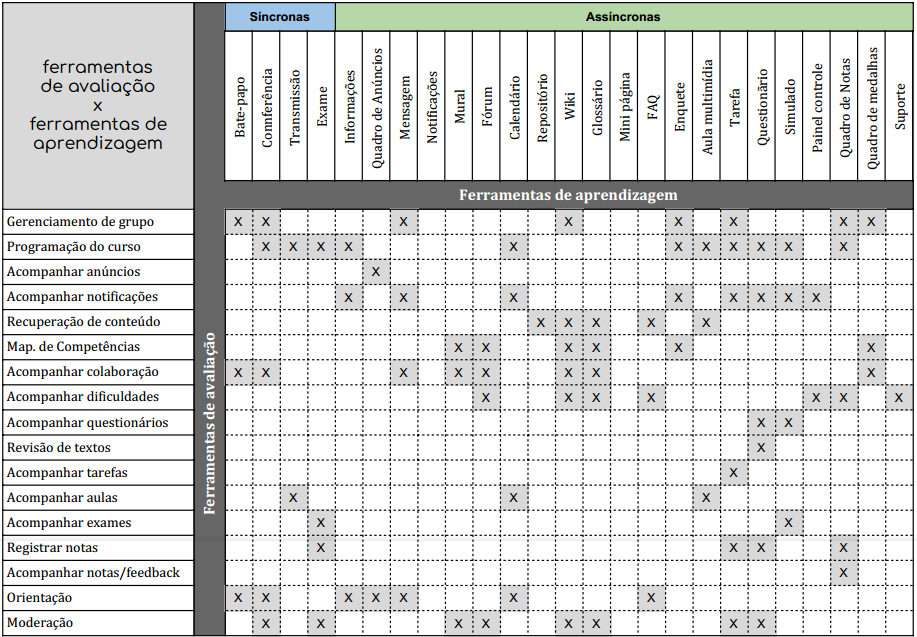
\includegraphics[width=\textwidth]{img/ferramentas_avaliacao.png}
        \caption{Tabela de vínculo entre ferramentas. Fonte: a autora.}
        \label{fig:ferramentas}
    \end{figure}
%\end{landscape}

\textbf{(--> A TABELA ESTÁ bastante confusa para o meu entendimento. Temos que conversar sobre isso. Como definiste o que é ferramenta de avaliação e ferramenta de aprendizagem? Algumas relações estão bastante difíceis de entender. Por exemplo, Programação do curso com transmissão e com enquete. Acredito que este é um aspecto que demandará bastante atenção do leitor, portanto as relações precisam estar muito claras para não haver dúvidas ou questionamentos. As ferramentas que o professor usa são consideradas de avaliação e a dos alunos de aprendizagem? Se for isso, precisas deixar bem claro como chegaste a esta tabela.)}  \textcolor{blue} {desculpe, estava com a legenda da primeira versão. foi corrigido. vou deixar para realizar alguma alteração quando conversarmos.}
Embora tenha sido criada para manter a rastreabilidade entre os dois perfis de ferramentas, nada impede que a tabela também possa ser utilizada de forma inversa. Por exemplo, dado que um determinado docente deseje realizar alguma atividade de avaliação com alguma das ferramentas de uso do professor, a tabela com os vínculos pode ser útil para identificar quais ferramentas precisam estar habilitadas no perfil do aluno. Nesse exemplo, podemos perceber que os registros de vínculos entre as ferramentas pode ser útil no planejamento das ações avaliativas, por antecipar os requisitos necessários para realizar a avaliação.

O levantamento das ferramentas do perfil do aluno e do professor, associado à tabela de vínculos compõe a listagem das ferramentas de AVA. As ferramentas de ambos os perfis foram listadas para esclarecer aspectos relevantes sobre as possibilidades de interação dentro desses ambientes. E, também, para identificar possíveis instrumentos de avaliação para o docente. Embora o levantamento tenha sido realizado com base nas funcionalidades disponíveis na plataforma Moodle e na plataforma BlackBoard, espera-se que ao menos uma parte delas esteja disponível em outras soluções. A seleção criteriosa desses dois ambientes teve a intenção de salvaguardar essa expectativa.

No próximo capítulo será proposta uma estratégia de mapeamento entre as ferramentas identificadas no perfil do professor com os tipos de avaliação estudados no \refCap{chap:ref}.

%Para exemplificar, tomemos como premissa que um determinado docente deseje realizar a atividade de avaliação denominada como ``Acompanhar dificuldades'', na qual ele utiliza dados parametrizados fornecidos pelo sistema para identificar se os discentes estão encontrando obstáculos no uso da plataforma. Para realizar essa avaliação, esse docente precisaria ter uma ou mais dessas ferramentas habilitadas: Fórum, Wiki, Glossário, FAQ e/ou Suporte.

%No caso em que esse mesmo docente não tenha habilitado nenhuma dessas ferramentas, a solução seria fazer um levantamento manual com a equipe para tentar identificar quais os problemas que os alunos mais reportaram. Ou, então, submeter algum tipo de consulta aos discentes para que esses informassem manualmente quais contratempos enfrentaram, tornando a atividade mais onerosa e passíveis de inconsistências.  O levantamento descritivo das ferramentas, associado à matriz de vínculos, pode gerar um catálogo das funcionalidades capazes de subsidiar a prática da avaliação em um AVA. Ainda, pode-se identificar a vinculação de uma ação avaliativa com sua função de avaliação, relacionando a ação com a intenção. 